\documentclass[10pt,a4paper]{article}
\usepackage[margin=18mm]{geometry}
\usepackage{amsmath,amssymb,booktabs,graphicx,array,xcolor,hyperref,fancyhdr,xurl}
\hypersetup{colorlinks=true,urlcolor=blue,linkcolor=black,pdftitle={Assignment 5: Optimising Attention on Apple M1}}
\setlength{\emergencystretch}{1.5em}\setlength{\parindent}{0pt}\setlength{\parskip}{5pt}\renewcommand{\arraystretch}{1.12}
\pagestyle{fancy}\fancyhf{}\lhead{CS6886: Systems for Deep Learning}\rhead{Assignment 5}\cfoot{\thepage}\setlength{\headheight}{13pt}
\newcommand{\question}[1]{\vspace{1mm}{\large\bfseries #1}\par\vspace{1mm}}
\begin{document}
{\LARGE\bfseries Optimising attention on Apple M1}\par
{\small Native MacBook Air measurements, 6 November 2026 \hfill CS6886, IIT Madras}

At $N=4096,d=64$, naive attention takes 1836.944 ms. The best single-threaded
variant takes 80.528 ms (22.81$\times$ faster), and 8 OpenMP threads take
26.335 ms (69.75$\times$ faster). All supplied-input checks and 72 independent
FP64 checks pass. The C kernels use no BLAS or external vector-math library.

\question{Q1. Machine and peak calculations}
The machine is a MacBook Air (MacBookAir10,1), with an Apple M1 and 16 GiB unified memory.
Native \texttt{sysctl} confirms four performance (P) cores and four efficiency (E) cores,
eight physical/logical cores and no SMT. All timings are native arm64 on macOS 15.1.1,
using Homebrew Clang 23.1.5 with \texttt{-O3 -mcpu=apple-m1 -fopenmp-simd};
only the OpenMP variant enables parallel OpenMP regions with \texttt{-fopenmp}.
\begin{center}
\footnotesize
\begin{tabular}{lp{111mm}}
\toprule
Property & Value / evidence \\
\midrule
Core types & Firestorm P + Icestorm E; 4 of each (native probe; Apple [1]) \\
SIMD / registers & 128-bit NEON, 4 FP32 lanes; 32 architectural vector registers \\
FMLA throughput & P: 4/cycle; E: 2/cycle (instruction microbenchmarks [2]) \\
Clock reference & P: 3.204 GHz; E: 2.064 GHz, platform operating points [3] \\
Base / sustained clock & DVFS; collected sysctl does not expose run-time core clocks \\
L1D / L1I per P core & 128 KiB / 192 KiB (native perflevel0 sysctl) \\
L1D / L1I per E core & 64 KiB / 128 KiB (native perflevel1 sysctl) \\
L2 clusters & 12 MiB shared by 4 P cores; 4 MiB shared by 4 E cores \\
L3 / cache line & Conventional L3 not reported; system cache unprobed / 128 B \\
Memory & 16 GiB unified; LPDDR4X-4266 platform reference [4] \\
\bottomrule
\end{tabular}
\end{center}

An FMA counts as two operations. Using the platform maximum operating points, the reference peaks are
\begin{align*}
P_P&=3.204\times4\times4\times2=102.528\;\mathrm{GFLOP/s},\\
P_E&=2.064\times2\times4\times2=33.024\;\mathrm{GFLOP/s},\\
P_{all}&=4P_P+4P_E=542.208\;\mathrm{GFLOP/s}.
\end{align*}
These are conditional architectural upper bounds, \emph{not measured sustained clocks}. The
P operating point appears as a turbo entry in the Linux/Asahi platform description; its Linux
availability does not establish which macOS frequency was used. A fixed base/all-core frequency
cannot be reported from this run. Percent-of-peak uses $P_P$ for serial variants; OpenMP uses
$P(t)=\min(t,4)P_P+\max(0,t-4)P_E$, a P-first reference model, not verified core placement.

For the platform memory model, use a 128-bit aggregate interface (two 64-bit-equivalent widths):
$B_{ref}=4266\times16/1000=68.256$ GB/s. Memory type/rate come from platform
identification [4]; the bus width is an explicit model assumption, not a probe of physical
LPDDR subchannels. A 384 MiB triad measures useful bandwidth as $B=12n/t$ (two reads plus
one FP32 write), excluding cached-store write allocation. The one-thread rate is 50.552 GB/s;
the best is 52.449 GB/s at two threads; eight threads give 42.991 GB/s.
Using measured bandwidth, the reference ridge points are $P_P/B_1=2.028$ and
$P_{all}/B_8=12.612$ FLOP/B. With theoretical $B_{ref}$, they are
1.502 and 7.944 FLOP/B.
\newpage
\question{Q2. Naive baseline}
\begin{center}
\small
\begin{tabular}{lrrrrrr}
\toprule
Variant & $N$ & $d$ & Time (ms) & GFLOP/s & \% peak$^\ast$ & vs naive \\
\midrule
naive & 1024 & 64 & 109.357 & 2.45 & 2.39 & 1.00$\times$ \\
naive & 2048 & 64 & 451.060 & 2.38 & 2.32 & 1.00$\times$ \\
naive & 4096 & 64 & 1836.944 & 2.34 & 2.28 & 1.00$\times$ \\
naive & 4096 & 128 & 3947.960 & 2.18 & 2.12 & 1.00$\times$ \\
\bottomrule
\end{tabular}
\end{center}

The common work count is $F=4N^2d$: $2N^2d$ for $QK^T$ and $2N^2d$ for the value product.
Reported throughput is $F/(10^9t)$. Softmax, division, key transposition and allocation remain
in the time but not the useful-work numerator, following the starter driver.

At $d=64$, doubling $N$ multiplies time by 4.12 and 4.07, close to the quadratic
prediction of 4. At $N=4096$, doubling $d$ multiplies time by 2.15: the products double
in work, while softmax still handles $N^2$ scores. Different cache/stride behaviour also matters.

The baseline computes each score as a separate dot reduction. Strict FP32 summation leaves
a dependent addition chain. Its value product uses $i,k,j$ loops, so $V[jd+k]$ is read with
a 256 B stride at $d=64$ and 512 B at $d=128$. The same probability row is traversed for
every output feature. This wastes locality and exposes reductions rather than independent
contiguous SIMD updates. These are code-based explanations; no per-stage timings or hardware
miss counters were collected on the Mac, so exact shares are not claimed.

\textbf{Protocol.} Every original starter driver is preserved. Each invocation performs one warm-up
and takes the median of five timed calls; the CSV is the median of three independently warmed
invocations per configuration. Only \texttt{attention()} is timed; file I/O is excluded, while all
temporary allocations and packing are included. Configurations run sequentially. macOS owns
P/E placement; no CPU affinity or fixed core frequency is claimed. Three-trial ranges on the
time plots are variability indicators, not confidence intervals.
\begin{center}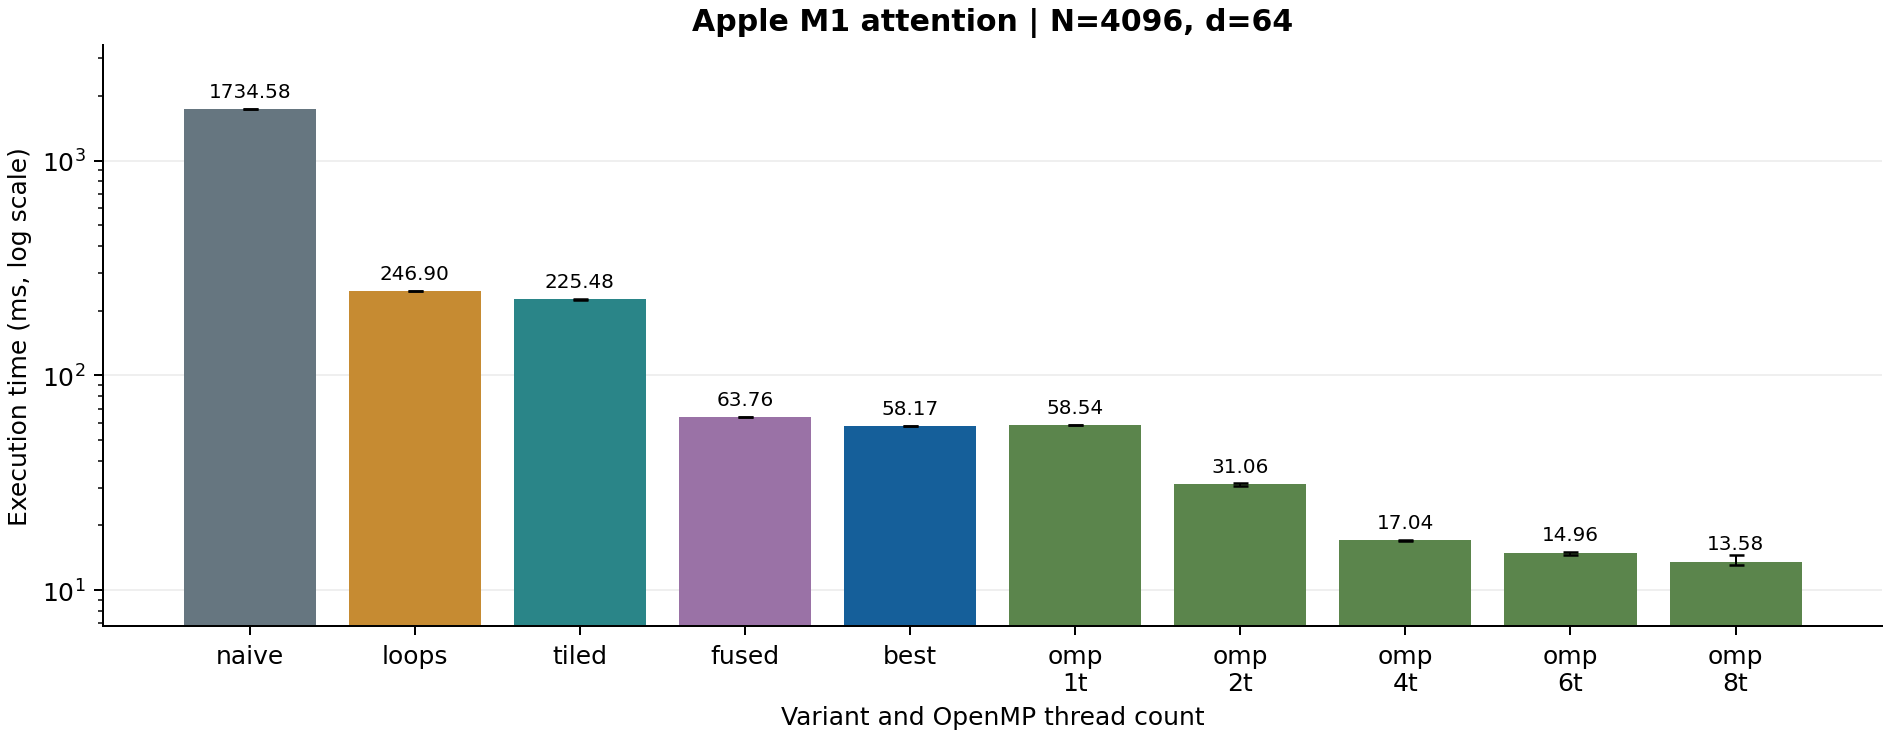
\includegraphics[width=0.98\linewidth]{plots/time_N4096_d64.png}\end{center}
The full CSV contains every input/variant/thread configuration. All four required per-input
time plots are supplied. One noisy invocation cannot change a row to its best-case time:
the report consistently uses the three-invocation median.
\vfill
{\footnotesize $^\ast$ Peak percentages refer to the Q1 reference architecture/frequency model.
GB and GFLOP use decimal units; KiB/MiB/GiB use binary units.}
\newpage
\question{Q3. Single-threaded variants}
\begin{center}
\small
\begin{tabular}{lrrrrrr}
\toprule
Variant & $N$ & $d$ & Time (ms) & GFLOP/s & \% peak$^\ast$ & vs naive \\
\midrule
loops & 1024 & 64 & 15.915 & 16.87 & 16.45 & 6.87$\times$ \\
loops & 2048 & 64 & 63.403 & 16.94 & 16.52 & 7.11$\times$ \\
loops & 4096 & 64 & 260.289 & 16.50 & 16.09 & 7.06$\times$ \\
loops & 4096 & 128 & 419.289 & 20.49 & 19.98 & 9.42$\times$ \\
tiled & 1024 & 64 & 14.370 & 18.68 & 18.22 & 7.61$\times$ \\
tiled & 2048 & 64 & 60.017 & 17.89 & 17.45 & 7.52$\times$ \\
tiled & 4096 & 64 & 239.650 & 17.92 & 17.48 & 7.67$\times$ \\
tiled & 4096 & 128 & 422.245 & 20.34 & 19.84 & 9.35$\times$ \\
fused & 1024 & 64 & 15.761 & 17.03 & 16.61 & 6.94$\times$ \\
fused & 2048 & 64 & 63.077 & 17.02 & 16.60 & 7.15$\times$ \\
fused & 4096 & 64 & 271.943 & 15.79 & 15.40 & 6.75$\times$ \\
fused & 4096 & 128 & 421.148 & 20.40 & 19.89 & 9.37$\times$ \\
best & 1024 & 64 & 5.175 & 51.87 & 50.59 & 21.13$\times$ \\
best & 2048 & 64 & 19.304 & 55.62 & 54.25 & 23.37$\times$ \\
best & 4096 & 64 & 80.528 & 53.34 & 52.02 & 22.81$\times$ \\
best & 4096 & 128 & 137.706 & 62.38 & 60.84 & 28.67$\times$ \\
\bottomrule
\end{tabular}
\end{center}

\textbf{(a) Reordered loops.} Transpose keys to $T[k,j]$ and use $i,k,j$ score loops. Adjacent
key positions become independent SIMD lanes. For $SV$, use $i,j,k$ so each probability
updates contiguous output features from a contiguous row of $V$. This removes strided
column access, but repeatedly updates score/output accumulators and retains the full score matrix.

\textbf{(b) Cache/register tiling.} Use $32\times128$ outer query/key tiles around $4\times32$
local accumulator tiles. Four query rows reuse each key/value vector; complete reductions
are kept in accumulators before storing results. It improves the $4096\times64$ case, but is
slightly slower than loops at $4096\times128$ (422.245 vs 419.289 ms). Tiling therefore has
shape-dependent benefits; local-array/control overhead can offset cache reuse. The difference
is small and is not evidence of a fundamental regression without more trials.

\textbf{(c) Row fusion.} Compute one score row, stable softmax, and its output immediately.
At $N=4096$, score storage falls from 64 MiB to 16 KiB. This version is still slower than
tiled at $d=64$: per-score dot reductions and lost multi-query reuse offset the storage saving.
At $d=128$, loops/tiled/fused are all around 419--422 ms, rather than monotonically improving.

\textbf{(d) Best M1 implementation.} Fuse blocks of 16 query rows; each NEON microkernel handles
four query rows by 16 keys/features, using sixteen independent 128-bit accumulators. Reuse
each loaded key/value vector across four queries and keep partial sums in registers.
A custom vector exponential accelerates stable softmax. At $N=4096$, each block needs 256 KiB
scratch, alongside 1 MiB of transposed keys and 1 MiB of values ($d=64$), fitting the P-cluster
L2. Packing is still timed. Scalar tails handle odd dimensions; the AArch64 fast path was
actually exercised in the submitted native Mac run. This is the best implemented/tested
variant, without a claim of global optimality or a measured M1 block-size search.

The remaining limits include FMA/load/broadcast throughput, softmax, packing, cache traffic
and OS scheduling. Exact bottleneck shares would require profiling beyond this run.
\newpage
\question{Q4. OpenMP}
The same compute kernel is used in \texttt{best} and \texttt{omp}. Key transposition is parallelised
over two-dimensional tiles. Query blocks use \texttt{schedule(dynamic,1)}: workers own private
scratch and disjoint output rows, and read shared keys/values. Dynamic block assignment lets
faster workers take more work on the asymmetric 4P+4E CPU. There is no cross-thread output reduction.

The controller disables dynamic team resizing and core binding. Thread placement remains
OS-managed. Define $S_t=T_{omp,1}/T_{omp,t}$ and $E_t=S_t/t$, using the one-thread OpenMP
implementation as the scaling baseline rather than the separately compiled serial binary.
\begin{center}
\footnotesize
\begin{tabular}{lrrrrrr}
\toprule
$N$ & $d$ & Threads & Time (ms) & GFLOP/s & $S_t$ & $E_t$ (\%) \\
\midrule
1024 & 64 & 1 & 4.832 & 55.55 & 1.000 & 100.0 \\
1024 & 64 & 2 & 2.668 & 100.61 & 1.811 & 90.6 \\
1024 & 64 & 4 & 1.838 & 146.05 & 2.629 & 65.7 \\
1024 & 64 & 6 & 1.615 & 166.21 & 2.992 & 49.9 \\
1024 & 64 & 8 & 1.592 & 168.62 & 3.035 & 37.9 \\
2048 & 64 & 1 & 19.073 & 56.30 & 1.000 & 100.0 \\
2048 & 64 & 2 & 11.031 & 97.34 & 1.729 & 86.5 \\
2048 & 64 & 4 & 8.239 & 130.32 & 2.315 & 57.9 \\
2048 & 64 & 6 & 9.520 & 112.79 & 2.003 & 33.4 \\
2048 & 64 & 8 & 5.773 & 185.99 & 3.304 & 41.3 \\
4096 & 64 & 1 & 83.119 & 51.67 & 1.000 & 100.0 \\
4096 & 64 & 2 & 48.953 & 87.74 & 1.698 & 84.9 \\
4096 & 64 & 4 & 33.710 & 127.41 & 2.466 & 61.6 \\
4096 & 64 & 6 & 31.112 & 138.05 & 2.672 & 44.5 \\
4096 & 64 & 8 & 26.335 & 163.09 & 3.156 & 39.5 \\
4096 & 128 & 1 & 155.675 & 55.18 & 1.000 & 100.0 \\
4096 & 128 & 2 & 85.504 & 100.46 & 1.821 & 91.0 \\
4096 & 128 & 4 & 60.493 & 142.00 & 2.573 & 64.3 \\
4096 & 128 & 6 & 64.284 & 133.62 & 2.422 & 40.4 \\
4096 & 128 & 8 & 57.451 & 149.52 & 2.710 & 33.9 \\
\bottomrule
\end{tabular}
\end{center}

For $N=4096,d=64$, eight threads yield 3.156$\times$ scaling and
39.5\% efficiency, or 69.75$\times$ over naive.
Eight identical full-speed cores would suggest an 8$\times$ line, but this CPU has four slower
E cores, shared caches/memory and scheduling overhead. That line is context, not an achievable
P-core-only target. Six threads are slower than four for $2048\times64$ and $4096\times128$;
eight are fastest for all four supplied shapes. The measurements show non-monotonic scaling,
not which thread was on which core. Contention, dynamic scheduling, placement and thermal/DVFS
effects are plausible contributors, not separately established causes.
\newpage
\question{Q5. Roofline}
\begin{center}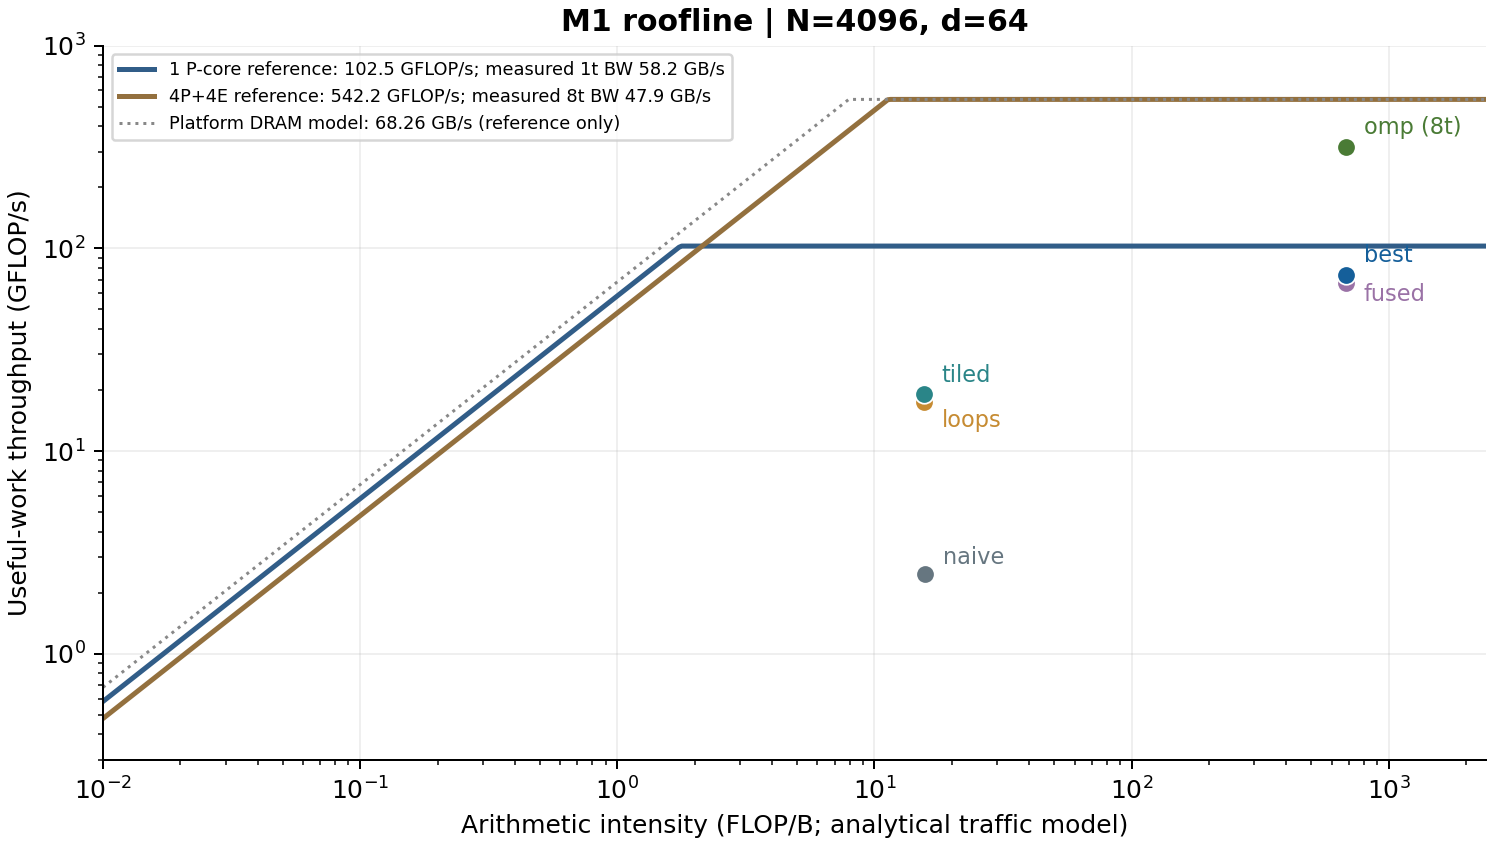
\includegraphics[width=0.98\linewidth]{plots/roofline.png}\end{center}

\textbf{Analytical traffic model.} Start with $16Nd$ bytes for reading $Q,K,V$ and writing $O$.
For materialised scores, add $16N^2$ bytes across stages: score write, softmax read/write,
then value-product read. Softmax's internal row passes are assumed to hit cache. A transposed
key buffer adds a conservative $8Nd$ bytes for its write/read. Fused row/block scratch is
assumed cache-resident. Ignore write allocation and additional evictions. Hence these
idealised intensities are not measured DRAM traffic and may overestimate actual intensity.
\begin{center}
\footnotesize
\begin{tabular}{llrr}
\toprule
Variant & Modelled bytes & $I=F/B$ (FLOP/B) & GFLOP/s \\
\midrule
naive & $16N^2+16Nd$ & 15.754 & 2.34 \\
loops & $16N^2+24Nd$ & 15.634 & 16.50 \\
tiled & $16N^2+24Nd$ & 15.634 & 17.92 \\
fused & $16Nd$ & 1024.000 & 15.79 \\
best & $24Nd$ & 682.667 & 53.34 \\
omp (8t) & $24Nd$ & 682.667 & 163.09 \\
\bottomrule
\end{tabular}
\end{center}

The rooflines use $\min(BI,P)$ with Q1's reference peak and either measured sustained bandwidth
or the explicitly assumed platform memory model. Serial points belong against the one-P-core
curve; the OpenMP point uses the 4P+4E curve. All points are beyond the corresponding ridge.
Thus modelled DRAM bandwidth is not the tight ceiling; this does not prove the kernels are
purely compute-bound. Naive suffers reduction/stride/cache-level costs; loops exposes SIMD
but repeats accumulator traffic; tiled reuses accumulators. Fused improves storage without
equivalent multi-row arithmetic reuse. Best adds explicit SIMD/register tiling and faster
softmax. OpenMP raises throughput but does not saturate the aggregate reference peak.
\newpage
\question{Validation, auxiliary measurements and reproduction}

\textbf{Validation.} All 36 non-reference input/configuration rows pass the required
$\max|O-O_{naive}|/\max|O_{naive}|\le10^{-4}$, including all 20 OpenMP configurations.
The worst supplied-input error is 4.73e-06. All 72 independent FP64 checks pass, with a
worst error of 4.16e-06; these include odd shapes, tails, zero/uniform logits and large logits.
SHA-256 matches all returned C/header sources and four original inputs to the packaged files.
The original naive source and all starter drivers are preserved. \texttt{make check} rejects
missing outputs, invalid headers/lengths, non-finite values and excessive error.

\textbf{Vector softmax approximation.} Subtract the row maximum, then reduce $x=n\ln2+r$ with
$n=\operatorname{round}(x\log_2e)$ and $|r|\le\ln2/2$. Evaluate
$e^x\approx2^n\sum_{k=0}^7r^k/k!$ with NEON FMAs. Values below $-87$ are set to zero
(each contribution below $1.65\times10^{-38}$); scalar tails use \texttt{expf}. The first omitted
polynomial term is below $5.2\times10^{-9}$, but final accuracy also includes FP32 range-reduction,
FMA and summation rounding. Output checks establish tolerance on the tested cases, not exactness.
\begin{center}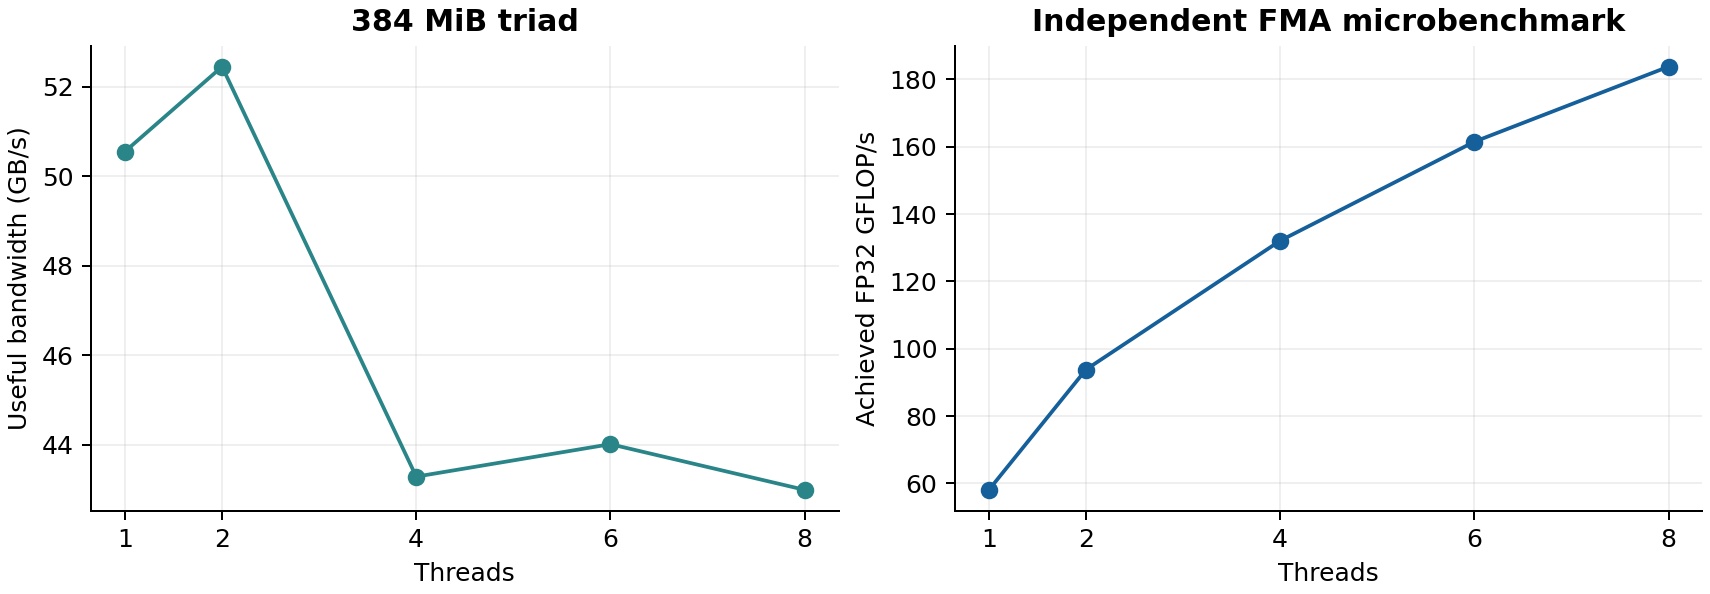
\includegraphics[width=0.98\linewidth]{plots/microbenchmarks.png}\end{center}
\begin{center}
\footnotesize
\begin{tabular}{lrr}
\toprule
Threads & Triad GB/s & Achieved FMA GFLOP/s \\
\midrule
1 & 50.552 & 58.076 \\
2 & 52.449 & 93.812 \\
4 & 43.286 & 132.074 \\
6 & 44.011 & 161.481 \\
8 & 42.991 & 183.784 \\
\bottomrule
\end{tabular}
\end{center}

The FMA test runs sixteen independent NEON chains, one warm-up and five measurements, counting
$16\times4\times2$ FLOPs per iteration per thread. It reports achieved rates, not a hard roof:
one attention shape exceeds its one-thread rate because instruction mix, timing and operating
conditions differ. The triad's best bandwidth occurs at two threads; more workers add contention
and scheduling costs rather than increasing the measured useful byte rate. No cache-miss,
power or sustained-frequency counters were collected.

\textbf{Reproduce.} On the M1, install Homebrew LLVM/libomp/Python, then run
\texttt{bash src/run\_macos.sh}. It compiles the kernels, runs all configurations/checks and
collects a result ZIP. \texttt{make all; make check} gives the starter-style workflow.
\texttt{python3 src/finalize\_mac.py} rebuilds this PDF, CSV/specification and plots from the
included native evidence (requires Matplotlib, NumPy and pdflatex). Use \texttt{--data PATH}
to supply another complete native run. Regeneration validates source hashes and raw medians.

Native evidence is under \path{src/evidence/mac_run/}. Local root paths are shortened
for portability. The main CSV preserves the measured
columns and adds clearly labelled reference-peak percentages. No earlier cloud timings,
stage-profile figures or tuning measurements are mixed into the Mac report.
\newpage
\question{References and run trace}
[1] Apple, MacBook Air (M1, 2020) technical specifications.

\url{https://support.apple.com/en-us/111883}

[2a] Dougall Johnson, Apple Microarchitecture Research: Firestorm SIMD/FP, FMLA vector 4S (0.25 cycles per instruction).

\url{https://dougallj.github.io/applecpu/firestorm-simd.html}

[2b] Dougall Johnson, Icestorm SIMD/FP, FMLA vector 4S (0.5 cycles per instruction). These are primary reverse-engineering measurements, not Apple specifications.

\url{https://dougallj.github.io/applecpu/icestorm-simd.html}

[3] Asahi Linux contributors, Linux T8103 device tree: 3.204 GHz P turbo / 2.064 GHz E operating points; these are reference values, not observed macOS clocks.

\url{https://github.com/torvalds/linux/blob/master/arch/arm64/boot/dts/apple/t8103.dtsi}

[4] iFixit, M1 MacBook Pro and Air Teardowns: primary chip identification of LPDDR4X-4266. The report explicitly assumes a 128-bit aggregate interface for the theoretical bandwidth model.

\url{https://www.ifixit.com/News/46884/m1-macbook-teardowns-something-old-something-new}

[5] Apple, Tuning your code's performance for Apple silicon: asymmetric cores and scheduling.

\url{https://developer.apple.com/documentation/apple-silicon/tuning-your-code-s-performance-for-apple-silicon/}

[6] Assignment starter, commit 29f5b9bf4aa89f74f425b1797cc46cdb457f5569.

\url{https://github.com/NMJ0/Assignment-5-Systems-for-Deep-learning}


\question{What is measured, assumed or unavailable}
\begin{center}
\footnotesize
\begin{tabular}{lp{111mm}}
\toprule
Category & Treatment \\
\midrule
Measured & Native times, errors, cache sizes, RAM capacity, cores, compiler, triad/FMA rates \\
Reference model & P/E instruction throughput and maximum operating points; LPDDR4X interface model \\
Unavailable & Actual per-core placement and clocks under load, cache-miss counters, package power \\
Not inferred & Eight P cores; a guaranteed base/all-core frequency; per-stage timing shares \\
Not established & Global optimality, definitive causes of every scaling fluctuation \\
\bottomrule
\end{tabular}
\end{center}

The full package retains the exact native C sources rather than substituting a subsequently
modified kernel. To reproduce the submitted results, use the same compiler/flags and report
all new timings when conditions change. The native runner prints its progress and fails if
compilation or a numerical check fails. The original binary inputs remain under \texttt{input/}.
The public GitHub URL is a submission step; it is not a performance result and must be supplied
when the repository is published.
\end{document}
